\newpage
\section{Open-loop System}

\subsection{System Model}

The chemical process illustrated in Figure~\ref{fig:reactor_scheme} represents an axial dispersion tubular reactor, which incorporates diffusion, convection, and a first-order irreversible chemical reaction \autocite{levenspiel1998chemical}. The reactor is equipped with a recycle mechanism, allowing a fraction of the product stream to re-enter the reactor to ensure the consumption of any unreacted reactants. By applying first-principle modeling through relevant mass balance relations on an infinitesimally small section of the reactor, the reactor's dynamics can be described by a second-order parabolic PDE, which is a common class of PDEs used to characterize diffusion-convection-reaction systems \autocite{jensen1982bifurcation}. The resulting PDE that describe the reactor model are as follows:

\begin{equation}
    \dot{x}(\zeta, t) = D \partial_{\zeta \zeta} x(\zeta, t) - v \partial_\zeta x(\zeta, t) + k_r x(\zeta, t)
\end{equation}

with the following boundary conditions:
\begin{align}
    \begin{cases}
        &D \partial_\zeta x(0, t) - v x(0, t) = -v \left[ R x(1, t-\tau) + (1-R) u(t) \right] \\
        &\partial_\zeta x(1, t) = 0 \\
        &y(t) = x(1, t)
    \end{cases}
\end{align}

\begin{figure}[ht]
    \centering
    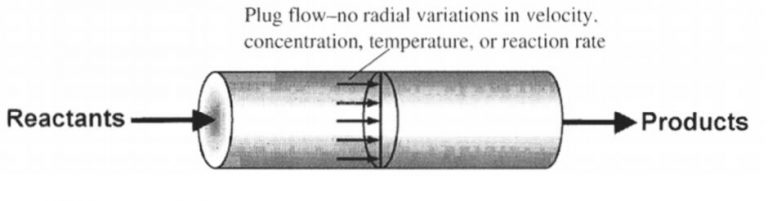
\includegraphics[width=0.7\textwidth]{Figures/sample.jpeg}
    \caption{Sample figure.}
    \label{fig:reactor_scheme}
\end{figure}